\section{Method}
\begin{figure}[h]
  \centering
  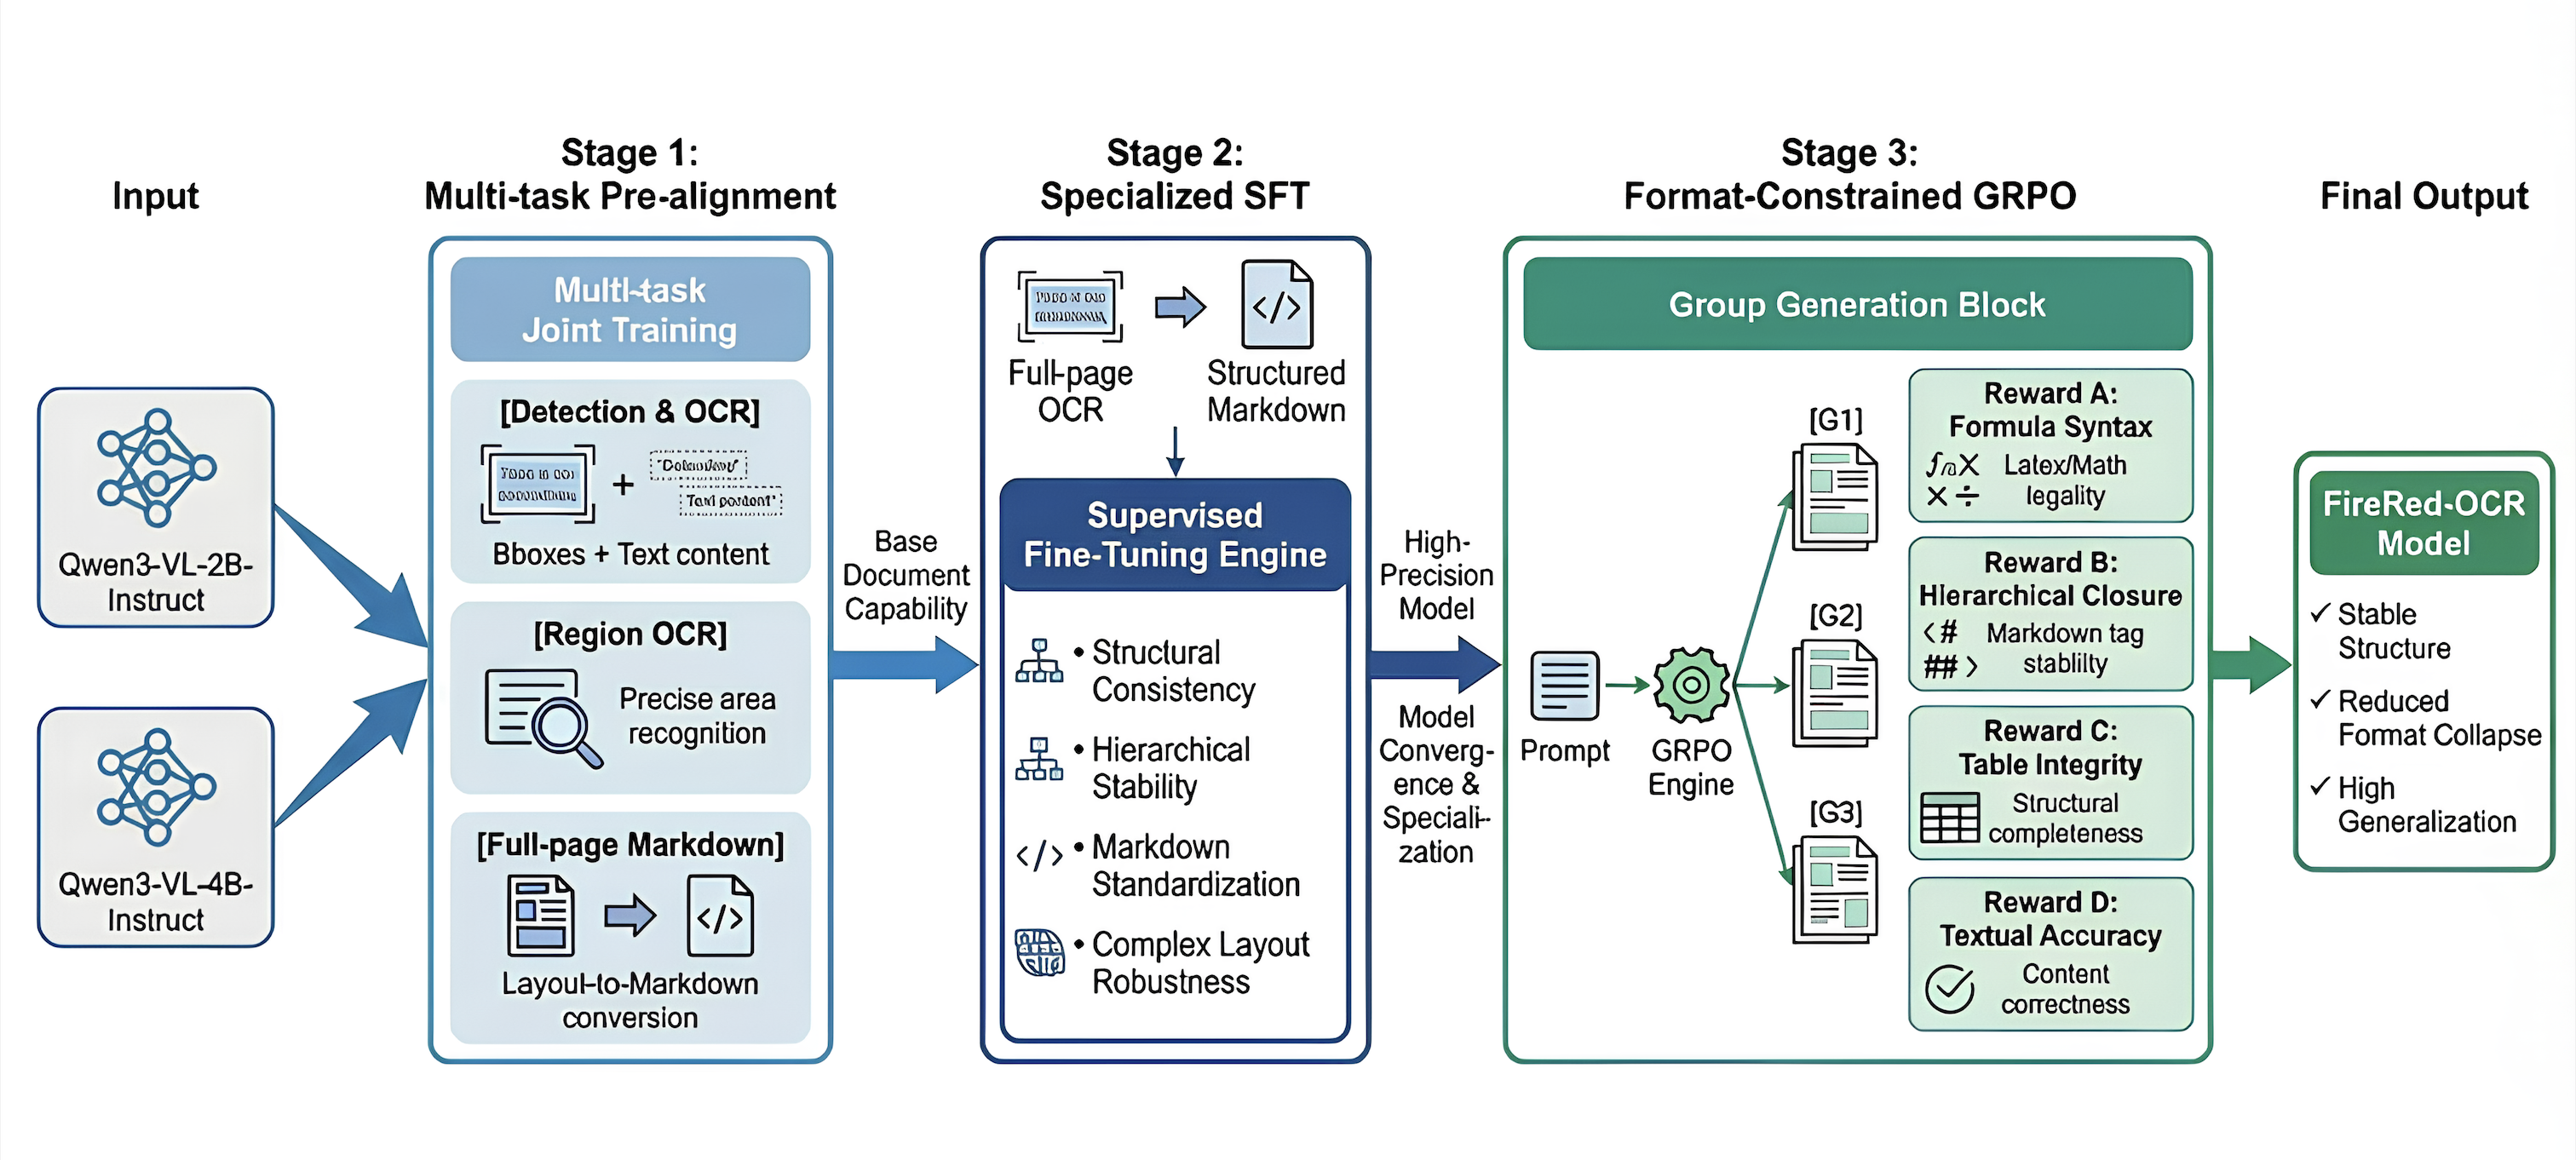
\includegraphics[width=0.99\textwidth]{figures/model.png}
  \caption{Overview of the FireRed-OCR training framework. The pipeline progresses through three stages: (1) Multi-task Pre-alignment, which employs joint training on detection, region OCR, and layout tasks to ground the model’s understanding of document structure; (2) Specialized Supervised Fine-Tuning (SFT), designed to adapt base capabilities for end-to-end structured Markdown generation; and (3) Format-Constrained GRPO, a reinforcement learning stage incorporating rule-based rewards (targeting formula syntax, hierarchical closure, and table integrity) to enforce structural compliance and textual accuracy.}
  \label{fig:pipeline}
\end{figure}

We propose \textbf{FireRed-OCR}, a coarse-to-fine progressive training framework designed to transform general-purpose Vision-Language Models (VLMs) into high-precision, structure-aware document understanding experts. As illustrated in Figure~\ref{fig:pipeline}, our pipeline utilizes the Qwen3-VL family as the backbone and proceeds through three distinct stages: \textit{Multi-task Pre-alignment}, \textit{Specialized Supervised Fine-Tuning (SFT)}, and \textit{Format-Constrained Group Relative Policy Optimization (GRPO)}.

\subsection{Stage 1: Multi-task Pre-alignment}
Standard VLMs often hallucinate in OCR tasks involving dense texts or complex layouts. To mitigate this, we first introduce a \textbf{multitask joint training} stage aimed at grounding the model's visual perception in fine-grained textual representations.

Let $\mathcal{D}_{pre}$ be the heterogeneous dataset comprising three distinct sub-tasks:
\begin{itemize}
    \item \textbf{Detection \& OCR ($\mathcal{T}_{det}$):} We train the model to output both bounding boxes and textual content simultaneously. Given an image $I$, the model predicts a sequence $S = \{ (b_i, t_i) \}$, where $b_i$ represents coordinates and $t_i$ is the recognized text. This forces the visual encoder to attend to precise spatial locations.
    \item \textbf{Region OCR ($\mathcal{T}_{reg}$):} To enhance local resolution sensitivity, we employ region-level recognition where the input includes a specific crop or coordinate prompt, and the output is the text within that region.
    \item \textbf{Full-page Markdown ($\mathcal{T}_{md}$):} We introduce initial layout-to-markdown conversion tasks to bridge the modality gap between visual layout and logical structure.
\end{itemize}

The objective function for Stage 1 is the standard auto-regressive cross-entropy loss over the combined dataset:
\begin{equation}
    \mathcal{L}_{Stage1} = - \sum_{(I, y) \in \mathcal{D}_{pre}} \sum_{t=1}^{T} \log P(y_t | y_{<t}, I; \theta_{base})
\end{equation}
This stage yields a model with "Base Document Capability," robust against perceptual errors but potentially lacking in structural formatting consistency.

\subsection{Stage 2: Specialized Supervised Fine-Tuning (SFT)}
Following the pre-alignment, the model possesses basic recognition capabilities but often struggles with the strict formatting required for downstream applications. To bridge this gap, Stage 2 employs \textbf{Specialized SFT} on a curated high-quality dataset $\mathcal{D}_{sft}$, specifically designed to transform raw OCR predictions into structured, machine-readable documents. The training emphasizes four critical dimensions to refine the "Base Document Capability" into a "High-Precision Engine":

\begin{itemize}
    \item \textbf{Structural Consistency:} We explicitly train the model to maintain logical coherence throughout long-context generation. This involves ensuring that the predicted sequence adheres to a valid Document Object Model, preventing fragmentation in lengthy documents.
    \item \textbf{Stability of Hierarchical Expression:} Special attention is given to the precise nesting of document structures. The model learns to strictly distinguish semantic levels, such as headers (e.g., \texttt{\#} vs. \texttt{\#\#}) and nested lists, ensuring the output faithfully reflects the visual hierarchy of the original layout.
    \item \textbf{Standardization of Markdown Formatting:} To mitigate the ambiguity inherent in natural language generation, we enforce a unified Markdown syntax. This involves canonicalizing representations for styling (e.g., bolding, italics) and mathematical expressions, thereby reducing variance in the output space and facilitating easier downstream parsing.
    \item \textbf{Robustness to Cross-lingual and Complex Layouts:} The training distribution is significantly broadened to include diverse linguistic scripts and challenging geometric topologies, such as dense multi-column scientific papers and mixed-media documents. This equips the model with the resilience to handle spatially complex and linguistically heterogeneous content without degradation in recognition accuracy.
\end{itemize}

Through this specialized tuning, the model effectively minimizes the structural hallucinations often observed in general-purpose VLMs, establishing a solid foundation for the subsequent reinforcement learning stage.

\begin{insight}[title=Insight 1: Benefits of Progressive Annotation Refinement.]
We discover that a \textit{coarse-to-fine} data strategy yields superior results compared to using the highest quality data throughout the entire training process. Specifically, training on coarser annotations (PaddleOCR-VL v1) in Stage 1 and finer annotations (v1.5) in Stage 2 achieves higher performance than using the high-precision v1.5 data for both stages.

This implies that coarser data provides a "smoother" learning landscape for the initial training phase, allowing the model to converge on general document understanding capabilities. Introducing the finer annotations later serves as a refinement step, preventing the model from getting stuck in local optima caused by the high complexity of fine-grained labels early in training.
\end{insight}

\subsection{Stage 3: Format-Constrained GRPO}
\label{sec:grpo}
The core innovation of FireRed-OCR is the application of \textbf{Group Relative Policy Optimization (GRPO)}~\cite{shao2024deepseekmath} with strictly defined format constraints. Unlike PPO~\cite{schulman2017proximal} which requires a separate Value model (doubling VRAM usage), GRPO estimates the baseline from the group average of generated outputs, making it highly efficient for high-resolution VLMs~\cite{bai2025qwen3,huang2026step3}.

\paragraph{Group Generation Block.}
For each prompt $x$ (an image-instruction pair), the model $\pi_\theta$ generates a group of $G$ outputs $\{o_1, o_2, ..., o_G\}$ by sampling. These outputs are then evaluated by a set of rule-based reward functions designed to penalize structural syntax errors.

\paragraph{Reward Engineering.}
We design a composite reward function $R(o)$ to guide the model towards structurally valid generation. The total reward is a weighted sum of four components:
\begin{equation}
    R(o) = \lambda_A r_{syntax} + \lambda_B r_{closure} + \lambda_C r_{table} + \lambda_D r_{text}
\end{equation}

\begin{enumerate}
    \item \textbf{Reward A: Formula Syntax ($r_{syntax}$):} We employ a lightweight \LaTeX\ parser/compiler check. If a generated formula string $\mathcal{F}$ fails to compile or contains illegal tokens, $r_{syntax} = -1$; otherwise, it provides a positive score based on complexity.
    \item \textbf{Reward B: Hierarchical Closure ($r_{closure}$):} This reward penalizes unclosed tags. For Markdown/HTML-like structures, or mismatched Markdown tags, we apply a penalty proportional to the number of open nodes. This enforces \textit{structural stability}.
    \item \textbf{Reward C: Table Integrity ($r_{table}$):} Tables are the most fragile structures in OCR. We parse the generated markdown table to check if the number of columns is consistent across all rows. $r_{table} = 1$ if the structure is rectangular and complete, else 0.
    \item \textbf{Reward D: Textual Accuracy ($r_{text}$):} While structure is key, content must remain faithful. We calculate the negative Levenshtein distance (normalized) between the generated text content (stripping structural tags) and the pseudo-ground truth from the SFT model (or human labels if available) to ensure \textit{content correctness}.
\end{enumerate}

\paragraph{Optimization Objective.}
The GRPO objective maximizes the following surrogate objective:
\begin{equation}
    \mathcal{J}_{GRPO}(\theta) = \mathbb{E}_{q \sim P(Q), \{o_i\}_{i=1}^G \sim \pi_{\theta_{old}}(o|q)} \left[ \frac{1}{G} \sum_{i=1}^G \min \left( \frac{\pi_\theta(o_i|q)}{\pi_{\theta_{old}}(o_i|q)} \hat{A}_i, \text{clip}\left(\frac{\pi_\theta(o_i|q)}{\pi_{\theta_{old}}(o_i|q)}, 1-\epsilon, 1+\epsilon\right) \hat{A}_i \right) \right] - \beta \mathbb{D}_{KL}
\end{equation}
where the advantage $\hat{A}_i$ is computed by normalizing the rewards within the group: $\hat{A}_i = \frac{R(o_i) - \text{mean}(\{R(o_j)\})}{\text{std}(\{R(o_j)\})}$.

By optimizing this objective, FireRed-OCR learns to navigate the trade-off between visual grounding and strict syntactic adherence, significantly reducing "Format Collapse" and achieving high generalization on unseen document types.

\begin{insight}[title=Insight 2: Synergistic Gains from Grounding Constraints.]
Interestingly, we observe that applying GRPO-based format constraints \textit{exclusively} to the grounding sub-task leads to a noticeable performance improvement in the main task. This suggests a spillover effect where the structural discipline required for precise coordinate prediction reinforces the model's overall visual-textual alignment. By forcing the model to be rigorous about "where" information is located, we implicitly enhance its ability to understand "what" the information is, thereby benefiting the primary generation task even without direct constraints.
\end{insight}

While the standard pipeline operates sequentially from Stage 1 to Stage 3, we introduce a cyclic refinement mechanism, denoted as \textbf{Iterative SFT-GRPO}. we observe that an iterative application of SFT and GRPO yields superior performance. In this paradigm, the model alternates between Specialized SFT (Stage 2) and Format-Constrained GRPO (Stage 3) for $K$ iterations.

We attribute the success of this iterative strategy to the synergistic interplay between likelihood-based instruction following and reward-based structural enforcement. Specifically:

\begin{enumerate}
    \item \textbf{Decoupling Semantic Fidelity from Structural Rigidity:} 
    FireRed-OCR faces a dual challenge: accurate text recognition (Semantic) and complex layout reconstruction (Structural). SFT primarily ensures the OCR content is correct (preventing hallucinations), while GRPO focuses on strict syntax compliance (e.g., ensuring \LaTeX{} formulas compile or Markdown tables have matching columns). Iterating between them allows the model to refine structural strictness without forgetting the underlying text recognition capabilities.
    
    \item \textbf{Mitigating Reward Hacking in Long-Context Generation:} 
    In pure RL training (GRPO), models may exploit the reward function by generating syntactically perfect but semantically empty or repetitive structures (reward hacking). By periodically re-introducing Specialized SFT using high-quality ground truth, we act as a regularizer that pulls the policy back towards the distribution of meaningful, content-rich document representations.
    
    \item \textbf{Progressive Hard-Constraint Adaptation:} 
    Learning complex constraints (such as hierarchical closure in nested lists or multi-row spanning cells in tables) is difficult in a single pass. The iterative cycle creates a curriculum: early iterations stabilize basic tag generation, while later iterations which guided by GRPO's specific rule-based rewards fine-tune the model to handle corner cases in document layout that standard SFT loss fails to capture.
\end{enumerate}